\chapter{ODE Data Representation}
In the Drasil framework, there is a single data structure containing all the information for all products, and we call it System Information. The giant System Information collects a multitude of pieces of information; whenever we need it, we extract the information from the System Information. In previous research, we store all ordinary differential equations (ODEs) information in the System Information. However, that information existed in the form of plain text. In other words, we explicitly wrote ODEs in the text without any advanced data structure. Although this method maintains the relationship of ODEs, it restricts any transformation of ODEs. For example, if the text-based ODE is higher-order linear ODE, we can not transform it to its equivalent system of first-order ODE. Therefore, the Drasil team is exploring new approach to store ODEs in a new data structure, and the new structure would allow ODEs be isomorphic, which means we can map the ODE from one form to other forms. Once we capture ODEs information in this data structure, we can generate its equivalent forms. This approach is contrasting to previous method, and it only requires users write ODEs once. This chapter we will introduce where the new data structure comes from, how the new data structure captures ODE information, how to use the new data structure, and how the new data structure interacts with the Drasil printer.

\section{Explicit Equation}
Before we conduct this research, the Drasil framework can generate software that provides numerical solutions for a first-order ODE by explicitly writing the equation. We re-write the ODE equation in a text-based form and pass it to the Drasil code generator. In Equation~\ref{eq_nopcmorginal}, the model describes the energy balance of water. In \href{https://jacquescarette.github.io/Drasil/examples/nopcm/SRS/srs/NoPCM_SRS.html#Sec:IMs}{NOPCM case study}, we can find the temperature of the water base on it.

\begin{equation} \label{eq_nopcmorginal}
	T_{w}'(t) +  \frac {T_{w}(t)}{\tau_{w}} = \frac{T_{c}}{\tau_{w}}
\end{equation}

The $T_w(t)$ is a function of the independent variable, in this case time. The $T_w$ is the temperature of water ($ ^\circ C $). The $T_w'(t)$ is the first directive of the function $T_w(t)$ respect time. The $T_c$ is the temperature of the heating coil (°C), and the $\tau_w$ is the ODE parameter for water related to decay time (s). We can later isolate the $T_w'(t)$ to the left-hand side and move the rest terms to the right-hand side. Then, we can get Equation~\ref{eq_nopcmderive}.
\begin{equation} \label{eq_nopcmderive}
	T_{w}'(t) = \frac{T_{c} - T_{w}(t)}{\tau_{w}}
\end{equation}

Based on Equation~\ref{eq_nopcmderive}, we can write it into a pure text-based form and pass it to the Drasil code generator. Code~\ref{code_expliciteq} shows how to encode Example~\ref{ex_firstorderode} by writing the explicit equation. We will discuss how to use explicit equations to get numerical solutions for ODEs in section~\ref{se_connecteetolib}.
\begin{listing}[ht]
\begin{haskell1}
-- Pesodu Code
reciprocal tau_w * (T_c - T_w[0])
\end{haskell1}
\captionof{listing}{NOPCM equation for the Drasil Code Generator}
\label{code_expliciteq}
\end{listing}

\begin{listing}[ht]
\begin{haskell1}
-- Pesodu Code
T_w'(t) = reciprocal tau_w * (T_c - T_w(t))
\end{haskell1}
\captionof{listing}{NOPCM equation for SRS}
\label{code_expliciteqsrs}
\end{listing}

In Code~\ref{code_expliciteq}, we encode Equation~\ref{eq_nopcmderive} in Drasil. Later, we will pass it to the Code Generator. The information is necessary for ODE libraries to solve the ODE numerically. In Code~\ref{code_expliciteqsrs}, we also encode Equation~\ref{eq_nopcmderive} and pass it to the Drasil printer. The information is necessary for printing ODEs in SRS. They both describe the same ODE, but we write it twice in the Drasil framework. Therefore, there is an information duplication. We can transform from Code~\ref{code_expliciteq} to Code~\ref{code_expliciteqsrs} with human interference. However, without human interference, we can not transfer between two expressions because they are all in a text-based form. To reduce the information duplication, the Drasil team decided to make an advanced data structure to hold the ODE information.

\section{Matrix Form}
In general, an equation contains a left-hand expression, a right-hand expression, and an equal sign. The left-hand and right-hand expressions connect by an equal sign. A linear ODE also has its left-hand and right-hand sides. Each side has its unique shape. We can write a linear ODE in the shape of

\begin{equation} \label{eq_matrixform}
	\boldsymbol{Ax} = \boldsymbol{b}
\end{equation}

On the left-hand side, \textbf{A} is an m $\times$ n matrix, and \textbf{x} is an n-vector. On the right-hand side, \textbf{b} is an m-vector. The \textbf{A} is commonly known as the coefficient matrix, \textbf{b} is the constant vector, and \textbf{x} is the unknown vector. The equation~\ref{eq_matrixform} can represent not only a single linear ODE, but also represent a linear system of ODE. A linear system of ODE is a finite set of linear differential equations. In this research, we only have case studies for single ODE, and all examples will demonstrate on single ODEs. The new data structure is capable to store information for a system of ODE, but its related functions only support for instances of single ODE.

Given the ODE example~\ref{eq_odeexmaple} in \href{https://jacquescarette.github.io/Drasil/examples/pdcontroller/SRS/srs/PDController_SRS.html#Sec:IMs}{PDContoller case study},
\begin{equation} \label{eq_odeexmaple}
	y_t''(t) + (1 + K_d) \cdot y_t'(t) + (20 + K_p) \cdot y_t(t) = r_t \cdot K_p
\end{equation}

In Example~\ref{eq_odeexmaple}, there is only one dependent variable $y_t$. The $y_t$(t) is a function of independent variable, in this case time. The $y_t'$(t) is the first derivative of $y_t$(t) respect time. The $y_t''$(t) is the second derivative of $y_t$(t) respect time. The $y_t$ is the process variable, and the $y_t'$ is the rate of change of $y_t$. The $y_t''$ is the rate of change of the rate of change of $y_t$. The $K_d$ , $K_p$, and $r_t$ are constant variables. The $K_d$ is Derivative Gain, $K_p$ is Proportional Gain, and $r_t$ is Set-Point. We can write this equation as follows.

\begin{equation} \label{eq_matrixformexmaple}
	\begin{bmatrix}
		1, & 1 + K_{d}, & 20 + K_{p}
	\end{bmatrix}
	\cdot
	\begin{bmatrix}
		y_{t}''(t)  \\
		y_{t}'(t)   \\
		y_{t}(t)  
	\end{bmatrix}
	=
	\begin{bmatrix}
		r_{t} \cdot K_{p} 
	\end{bmatrix}
\end{equation}

The relationship between the matrix form~\ref{eq_matrixform} and the example~\ref{eq_matrixformexmaple} is not hard to find. Firstly, the coefficient matrix \textbf{A} is a 1 $\times$ 3 matrix that consists of $1$, $1 + K_d$, ane $20 + K_p$. Secondly, the unknown vector \textbf{x} is a 3 $\times$ 1 vector with $y_t''$, $y_t'$, and $y_t$. Last, the constant vector \textbf{b} is a 1 $\times$ 1 vector with $r_t \cdot K_p$. The matrix form~\ref{eq_matrixform} very well captures all the knowledge we need to present an ODE. Therefore, we decided to create a datatype called \verb|DifferentialModel| to preserve ODEs information. The \verb|DifferentialModel| has six records, and here is the representing code for \verb|DifferentialModel|.
\begin{haskell1}
data DifferentialModel = SystemOfLinearODEs {
	_indepVar :: UnitalChunk,
	_depVar :: ConstrConcept,
	_coefficients :: [[Expr]],
	_unknowns :: [Unknown],
	_dmConstants :: [Expr],
	_dmconc :: ConceptChunk
}
\end{haskell1}

Previous to this research, UnitalChunk, ConstrConcept, Expr, and ConceptChunk already existed in Drasil. We created an \verb|Unknown| type for this experiment. Their semantics will show up in table ~\ref{tab_demodeltype}

\begin{table}[ht]
	\begin{tabular}{ p{0.2\textwidth} p{0.7\textwidth} }
		\textbf{Type} & \textbf{Semantics} \\
		\toprule
		\verb|UnitalChunk| & concepts with quantities that must have a unit definition.\\
		\verb|ConstrConcept| & conceptual symbolic quantities with Constraints and maybe a reasonable value.\\
		\verb|Expr| & a type encode mathematical expression. \\
		\verb|ConceptChunk| & a concept that contains an idea, a definition, and an associated domain of knowledge\\
        \verb|Unknown|& synonym of Integer\\
		\bottomrule	
	\end{tabular}	
	\caption{Type use in DifferentialModel}	
	\label{tab_demodeltype}
\end{table}

The \verb|_indepVar| represents the independent variable, and it is often time. The \verb|_depVar| represents the dependent variable. Combing \verb|_depVar| and \verb|_indepVar|, it represents a function produce dependent variables over time. The \verb|_coefficients| is a list of lists \verb|Expr|, and it represents the coefficient matrix \textbf{A}. The \verb|_unknowns| is a list of \verb|Unknown|, and \verb|Unknown| is synonym of integers.
The \verb|_unknowns| represent a list of numbers of derivatives of the function. Combining \verb|_depVar|, \verb|_indepVar| and \verb|_unknowns|, they can represent the unknown vector \textbf{x}. The \verb|_dmConstants| is a list of \verb|Expr|, and it represents the constant vector \textbf{b}. Last, the \verb|_dmconc| contains metadata of this model. To represent example~\ref{eq_odeexmaple} in \verb|DifferentialModel|, \verb|_indepVar| is time, \verb|_depVar| is $y_t$, \verb|_coefficients| is the 1 $\times$ 3 matrix, \verb|_unknowns| is the 3 $\times$ 1 vector, \verb|_dmConstants| is the 1 $\times$ 1 vector, and \verb|_dmconc| is \verb|ConceptChunk| that describes what this model is. Code~\ref{code_interaldata} shows the internal data representation of the example~\ref{eq_odeexmaple} in \verb|DifferentialModel|.

\begin{listing}[ht]
\begin{haskell1}
_indepVar = time
_depVar = y_t
_coefficients = [[1, 1 + K_d, 20 + K_p]]
_unknowns = [2, 1, 0]
_dmConstants = [r_t K_p]
_dmconc = ... -- Drasil definition for chuck concept
\end{haskell1}
\captionof{listing}{Internal Data Representation for the example~\ref{eq_odeexmaple}}
\label{code_interaldata}
\end{listing}

Currently, the \verb|DifferentialModel| only captures the knowledge of ODEs with one dependent variable, and it is a special case of the family of linear ODEs. Studying this special case will help the Drasil team better understand how to capture the knowledge of all ODEs and eventually lead to solving a system of linear ODE with multiple dependent variables. On top of that, there is one assumption. The \verb|_coefficients| can only be functions of independent variable, often time. In other word, the \verb|_coefficients| does not depend on \verb|_depVar|.

\section{Input Language}
\label{sec_input}
There are many reasons why we want to provide an input language for users to input ODE equations. One major reason is that it could be over complicated for users to input a single ODE in a matrix form. While inputting a single ODE, one obvious way is directly passing value to each record via constructors of \verb|DifferentialModel|. However, it would be not so elegant to set a single ODE in the example, because users have to extracts the coefficient matrix \textbf{A}, unknown vector \textbf{x} and constant vector \textbf{b} from the original equation manually. Once the coefficient matrix, unknown vector and constant vector is ready, we can set value into \verb|_depVar|, \verb|_coefficients|, \verb|_unknowns|, and \verb|_dmConstants| accordingly. This process is ideal when the ODE is a system of ODE, and it would be over-complicated for user to do extraction for a single ODE. Therefore, we decided create a helper function to ease this issue. Another advantage of having an helper function to input an ODE is that it can reduce human error and make sure the equation is well-formed. We call this helper function input language, and what will this input language looks like? The input language is inspired by how a linear nth-order ODE looks like. Based on Paul's Online Notes~\citep{paullinearode}, we can write all linear ODEs in the shape of 
\begin{equation} \label{eq_linearDE}
	a_n(t) \cdot y^n(t) + a_{n-1}(t) \cdot y^{n-1}(t) + \dots + a_1(t) \cdot y'(t) + a_0(t) \cdot y(t) = g(t)
\end{equation}

On the left-hand side of the linear equation~\ref{eq_linearDE}, the expression is a collection of terms. Each term consists of a coefficient and a derivative of the function y(t). With ideas of term, coefficient, and derivative, we create new data types to mimic the mathematical expression of a linear ODE. The following is the detail of the code for new data types and operators.

\begin{haskell1}
type Unknown = Integer
data Term = T{
	_coeff :: Expr,
	_unk :: Unknown
}
type LHS = [Term]

($^^) :: ConstrConcept -> Integer -> Unknown
($^^) _ unk' = unk'

($*) :: Expr -> Unknown -> Term
($*) = T

($+) :: [Term] -> Term -> LHS
($+) xs x  = xs ++ [x]
\end{haskell1}

For new types, the \verb|LHS|, the short name for the left-hand side, is a list of \verb|Term|. This corresponds to the left hand side is a collection of terms. Each \verb|Term| has an \verb|Expr| and \verb|Unknown|. This corresponds to a term consists of a coefficient and a derivative of the function. Although \verb|_unk| is an integer, combining \verb|_unk|, \verb|_depVar| and \verb|_indepVar| we can get the derivative of the function. For new operators, they are inspired by the linear equation~\ref{eq_linearDE}. The \verb|$^^| operator take a variable and a integer, and it represents the derivative of the function. For instance, in example~\ref{eq_odeexmaple}, we can write $y_t(t)$\^{}\^{}2 to represent $y_t''(t)$. One thing we want to notice here is that we store $y_t(t)$ in \verb|_depVar| and \verb|_indepVar|. The operator \verb|$^^| will ignore the first parameter, and store the second parameter in \verb|_unknowns|. The reason to positioning a dummy variable before \verb|$^^| is becasue this will maintain the whole input structure as close as a linear ODE. The \verb|$*| operator creates a term by combining a coefficient matrix and a derivative function. For instance, in example~\ref{eq_odeexmaple}, we can write $(1 + K_d) \$* (y_t$ \$\^{}\^{}1) to represent $(1 + K_d) \cdot y_t'(t)$. Last, the \verb|$+| operator will append all terms into a list. Let's write pseudo code (Code \ref{code_exinputl}) for the example matrix form~\ref{eq_odeexmaple} in the newly introduced input language. The full detail of the input language for the PDController example will show up in ~\ref{const_de}.

\begin{listing}[ht]
\begin{haskell1}
-- in example \ref{eq_odeexmaple}: y\_t'' + (1 + K\_d)y\_t' + (20 + K\_p)y\_t = r\_t K\_p
-- left hand side = y\_t'' + (1 + K\_d)y\_t' + (20 + K\_p)y\_t 
-- right hand side = r\_t K\_p

lhs = [1 $* (y_t $^^ 2)]
	$+ (1 + K_d) $* (y_t $^^ 1)
	$+ (20 + K_p) $* (y_t $^^ 0)
rhs = r_t K_p
\end{haskell1}
\captionof{listing}{Input language for the example~\ref{eq_odeexmaple}}
\label{code_exinputl}
\end{listing}

\section{Two Constructors}
There are many way to create the a \verb|DifferentialModel|. One most obvious way is to set each record directly by passing values in the constructor and \verb|makeASystemDE| constructor serve as this role. We also designed another constructor, \verb|makeASingleDE|, for users who want to use input language to create a \verb|DifferentialModel|.

For \verb|makeASystemDE| constructor, a user can set the coefficient matrix, unknown vector, and constant vector by explicitly giving \verb|[[Expr]]|, \verb|[Unknown]|, and \verb|[Expr]|. There will be several guards to check whether inputs are well-formed.

1. The coefficient matrix and constant vector dimension need to match. The \verb|_coefficients| is an m $\times$ n matrix, and \verb|_dmConstants| is an m vector. This guard makes sure they have the same m dimension. If an error says ``Length of coefficients matrix should equal to the length of the constant vector.'', it means \verb|_coefficients| and \verb|_dmConstants| has different m dimension, violating mathematical rules.

2. The dimension of each row in the coefficient matrix and unknown vector need to match. The \verb|_coefficients| use a list of lists to represent an m $\times$ n matrix. It means each list in \verb|_coefficients| will have the same length n, and \verb|_unknowns| is an n-vector. Therefore, the length of each row in the \verb|_coefficients| should equal the length of \verb|_unknowns|. If an error says, ``The length of each row vector in coefficients need to equal to the length of unknowns vector.'', it means \verb|_coefficients| and \verb|_unknowns| violate mathematical rules.

3. The order of the unknown vector needs to be descending due to design decisions. We have no control over what users will give to us, and there are infinite ways to represent a linear equation in the matrix form~\ref{eq_matrixform}. We strictly ask users to input the unknown vector descending, so we can maintain the shape of a normal form of linear ODE~\ref{eq_linearDE}. This design decision will simplify the implementation for solving a linear ODE numerically in Chapter 3. If an error says, ``The order of giving unknowns needs to be descending.'', it means the order of unknown vector is not descending.

The following pseudo-code shows how to directly set the example~\ref{eq_odeexmaple}'s coefficient matrix, unknown vector, and constant vector. The full detail of how to directly set the coefficient matrix, unknown vector, and constant vector for the \href{https://jacquescarette.github.io/Drasil/examples/pdcontroller/SRS/srs/PDController_SRS.html}{PDContoller} example will show up in the Appendix~\ref{const_de}.

\begin{haskell1}
coefficent = [[1, 1 + K_d, 20 + K_p]]
unknowns   = [2, 1, 0]
constants  = [r_t K_p]
\end{haskell1}

The second constructor is called \verb|makeASingleDE|. This constructor uses the input language to simplify the input of a single ODE. In \verb|makeASingleDE|, we create the coefficient matrix, unknown vector, and constant vector based on restricted inputs. In other words, users can no longer set the data by directly giving values. The \verb|DifferentialModel| will generate all data for the coefficient matrix, unknown vector, and constant vector accordingly. The constructor first creates a descending unknown vector base on the highest number of its derivatives. To take the code~\ref{code_exinputl} as an example, the highest order of its derivative on the left-hand side of the equation is 2, so we will generate the unknown vector, and it is a list that contains 2, 1 and 0. Then, we will create the coefficient matrix by finding its related coefficient based on the descending order of the unknown vector. The main advantage of this design decision is that the \verb|DifferentialModel| will no longer require users to input the unknown vector in descending order. Any order of the unknown vector will be acceptable because we will generate relative data in \verb|DifferentialModel|. The pseudo-code~\ref{code_exinputl} shows how to use the input language to set the example~\ref{eq_odeexmaple}'s coefficient matrix, unknown vector, and constant vector. The full detail of how to use the input language set the coefficient matrix, unknown vector, and constant vector for the \href{https://jacquescarette.github.io/Drasil/examples/pdcontroller/SRS/srs/PDController_SRS.html}{PDContoller} example will show up in the Appendix ~\ref{const_de}.

\section{Display Matrix}
After a \verb|DifferentialModel| obtains ODE information, we want to display them in the software requirements specification (SRS). Previously, we mentioned the Drasil framework able to generate software artifacts, and SRS is a part of them. This section will discuss two ways to display ODEs in the SRS.

\begin{figure}[ht]
	\centering
	\begin{subfigure}[t]{\textwidth}
		\centering
		
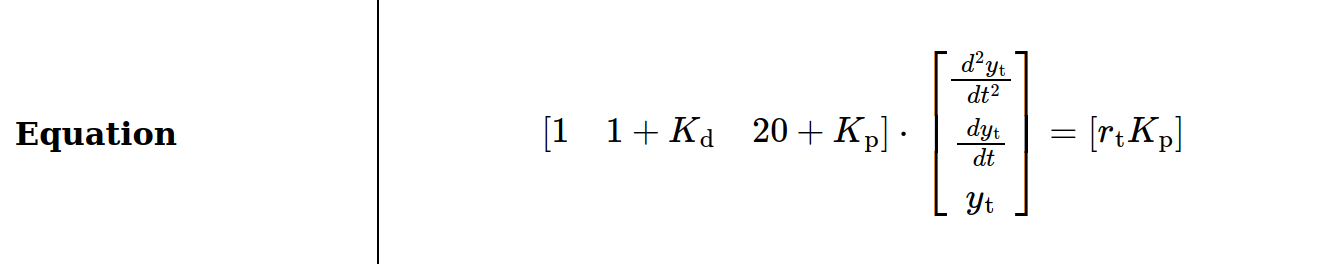
\includegraphics[width=1\textwidth]{figures/ODEInMatrix.png}
		\caption{Displaying ODE in a matrix form}
		\label{fig_multienv_odematrix}
	\end{subfigure}
	~
	\begin{subfigure}[t]{\textwidth}
		\centering
	
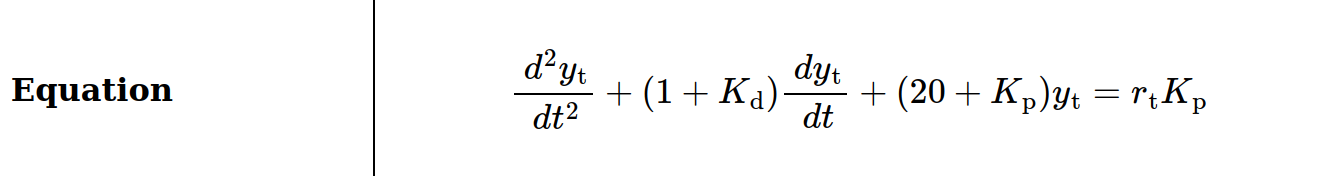
\includegraphics[width=1\textwidth]{figures/ODEInLinearEq.png}
		\caption{Displaying ODE in a linear equation}
		\label{fig_multienv_odelinear}
	\end{subfigure}
	
	\caption{Options of Displaying an ODE}
	\label{fig_multienv}
\end{figure}

1. We can display ODEs in a matrix form. The matrix form~\ref{eq_matrixformexmaple} demonstrates how the ODE will appear in a matrix form in the SRS. In the \verb|DifferentialModel|, the coefficient matrix is a list of lists expression, the unknown vector is a list of integers, and the constant vector is a list of expressions. It should be fairly straightforward for the Drasil printer to display them by printing each part sequentially. The example for this option shows in Figure~\ref{fig_multienv_odematrix}. However, we explicitly force the Drasil printer to display a single ODE in shape of a linear equation, because displaying a single ODE in matrix from would be over-complicated. The example is a demo shows the Drasil printer is capable to display an ODE in a matrix form.

2. We also can display ODEs in a shape of a linear equation. The example~\ref{eq_odeexmaple} demonstrates how the ODE will show up in the shape of a linear equation in the SRS. Displaying a single ODE in a linear equation is a special case. When there is only one single ODE, it would be over complicated to display it in a matrix form. This is the same reason we want to create an input language to manage the input of a single ODE better. The example for this option shows in Figure~\ref{fig_multienv_odelinear}.

In the future, the Drasil team wants to explore more variability in displaying ODEs. One topic highlighted in the discussion is showing an ODE in a canonical form. However, many mathematicians have different opinions on a canonical form, and the name of canonical form has been used differently, such as normal form or standard form. More research on this part would help us better understand the knowledge of ODE.
